\documentclass[11pt]{article}

\usepackage{footnote}
\usepackage{tablefootnote}
\usepackage{multicol}
\usepackage{graphicx}
\usepackage{url}
\usepackage{todonotes}

\begin{document}
\title{Identify Fraud from Enron Email}
\author{Jean Paul Barddal}
\maketitle

\section{Introduction}

	This report details the Enron Email Fraud Identification project that aims at building employees that committed fraud, namely the Persons of Interest (POIs).
	It discusses several basic tasks of machine learning, including (i) extracting basic information about the dataset, (ii) the creation of new attributes, (iii) outlier identification and removal, (iii) data scaling, (iv) classification tuning, and (v) evaluation metrics for classifier comparison.
	This report is based on a work that used scikit-learn (\url{http://scikit-learn.org/stable/}).

	This report is divided as follows.
	Section \ref{sec:about} introduces the data set and some of its characteristics.
	It also introduces the feature selection methods used and the results obtained.
	Later, it shows how outlier detection was performed, and how data was scaled prior to learning.	
	Section \ref{sec:results} shows the rationale behind the classifier tuning process adopted and the results obtained.
	It also includes a thorough discussion of the results obtained by classifiers used in (i) the original dataset, (ii) the original dataset with the new features and (iii) the dataset with the selected attributes.
	
	
\section{About the data set} \label{sec:about}

	\subsection{Original data set}
	
		The developed script gathers some basic information on the data set, such as:
		\begin{itemize}
			\item Number of instances = 146
			\item Number of POIs = 18
			\item Number of features = 21
			\item Ratio between POIs and non POIs = 12\%, 88\%
		\end{itemize}
		
		Therefore, this is a low-dimensionality data set, yet, is unbalanced.
		If one assumes a ZeroR learning scheme as a baseline, it would be necessary to achieve accuracies above 88\% to provide meaningful results.
		Roughly speaking, this occurs since classifiers, when applied over unbalanced data sets, will be biased towards the majority class, and if it forgets the minority class, and vote ''not a POI'' for each instance, it would obtained an 88\% accuracy.
	
	
	\subsection{Creating new features}
		Two new features were created: ``total\_asset'' and ``fraction\_of\_messages\_with\_poi''.
		The first is simple the sum of all the assets of an instance, i.e. ``salary'', ``bonus'', ``total\_stock\_value'' and ``exercised\_stock\_options'', while the second is the ratio between messages to and from a POI and all the messages.
	
	
	\subsection{Feature selection}
		The proposed method for feature selection was to maximize the F1-Weighted\footnote{F1-Weighted was used in replacement of F1 since the dataset is unbalanced.} metric of the selected subset of features given each classifier.
		In practice, this is mix between a step-wise and a wrapper-like approach, where attributes are selected sequentially (using SelectKBest) and evaluated using different classifiers.
		Using SelectKBest, features are selected regardind their direct correlation to the class.
		The evaluation using different classifiers is due that different classifiers work differently with different attributes.
		Table \ref{tab:selectedFeatures} presents the selected features for each classifier.

		\begin{table*}[!t]
			\centering
			\caption{Features selected for usage in each classifier.}
			\begin{tabular}{rl}
				\hline
				Learner & Features selected\\
				\hline
				Gaussian NB & \{exercised\_stock\_options\}\\
				SGD & \{salary, total\_payments, loan\_advances, bonus,\\
				~   & restricted\_stock\_deferred, deferred\_income,\\ 
				~   & total\_stock\_value, expenses, exercised\_stock\_options, \\
				~   & director\_fees, to\_messages, from\_poi\_to\_this\_person, \\
				~   & from\_messages, shared\_receipt\_with\_poi\}\\
				$k$NN & \{total\_payments, exercised\_stock\_options\}\\
				Decision Tree & \{salary, total\_payments, to\_messages\}\\
				\hline
			\end{tabular}
			\label{tab:selectedFeatures}
		\end{table*}
		
		Table \ref{tab:featureScores} presents the feature scores obtained using the SelectKBest method, while Figure \ref{fig:kVersusMetrics} shows the Precision, Recall and F1 metrics obtained by varying the $k$ parameter using the Gaussian NB classifier in the SelectKBest algorithm.
		In practice, the only $k$ parameter that achieves the required precision and recall results above $0.3$ is $k=1$, yet, $k=14$ achieves the best overall F1 measure, which is the harmonic mean between precision and recall (see Equation \ref{eq:f1} in Section \ref{sec:overallEvaluation}).
		
		\begin{table*}
			\caption{Features scores. Bold faced features represent the newly generated attributes.}
			\begin{center}			
			\begin{tabular}{rl}
				\hline
				Feature & Score \\
				\hline
				exercised\_stock\_options & 24.81507973\\
				total\_stock\_value & 24.17997245\\
				bonus & 20.79225205\\
				salary & 18.28968404\\
				\textbf{total\_asset} & \textbf{15.36927686}\\
				deferred\_income & 11.45847658\\
				long\_term\_incentive & 9.92218601\\
				restricted\_stock & 8.82867901\\
				total\_payments & 8.77277773\\
				shared\_receipt\_with\_poi & 8.58942073\\
				loan\_advances & 7.18405566\\
				expenses & 6.09417331\\
				\textbf{fraction\_of\_messages\_with\_poi} & \textbf{5.39937029}\\
				from\_poi\_to\_this\_person & 5.24344971\\
				other & 4.18747751\\
				from\_this\_person\_to\_poi & 2.38261211\\
				director\_fees & 2.1263278\\
				to\_messages & 1.64634113\\
				restricted\_stock\_deferred & 0.24705326\\
				deferral\_payments & 0.23309098\\
				from\_messages & 0.16970095\\
			   	\hline
			\end{tabular}
			\end{center}			
			\label{tab:featureScores}
		\end{table*}

		\begin{figure}
			\resizebox{\textwidth}{!}{
				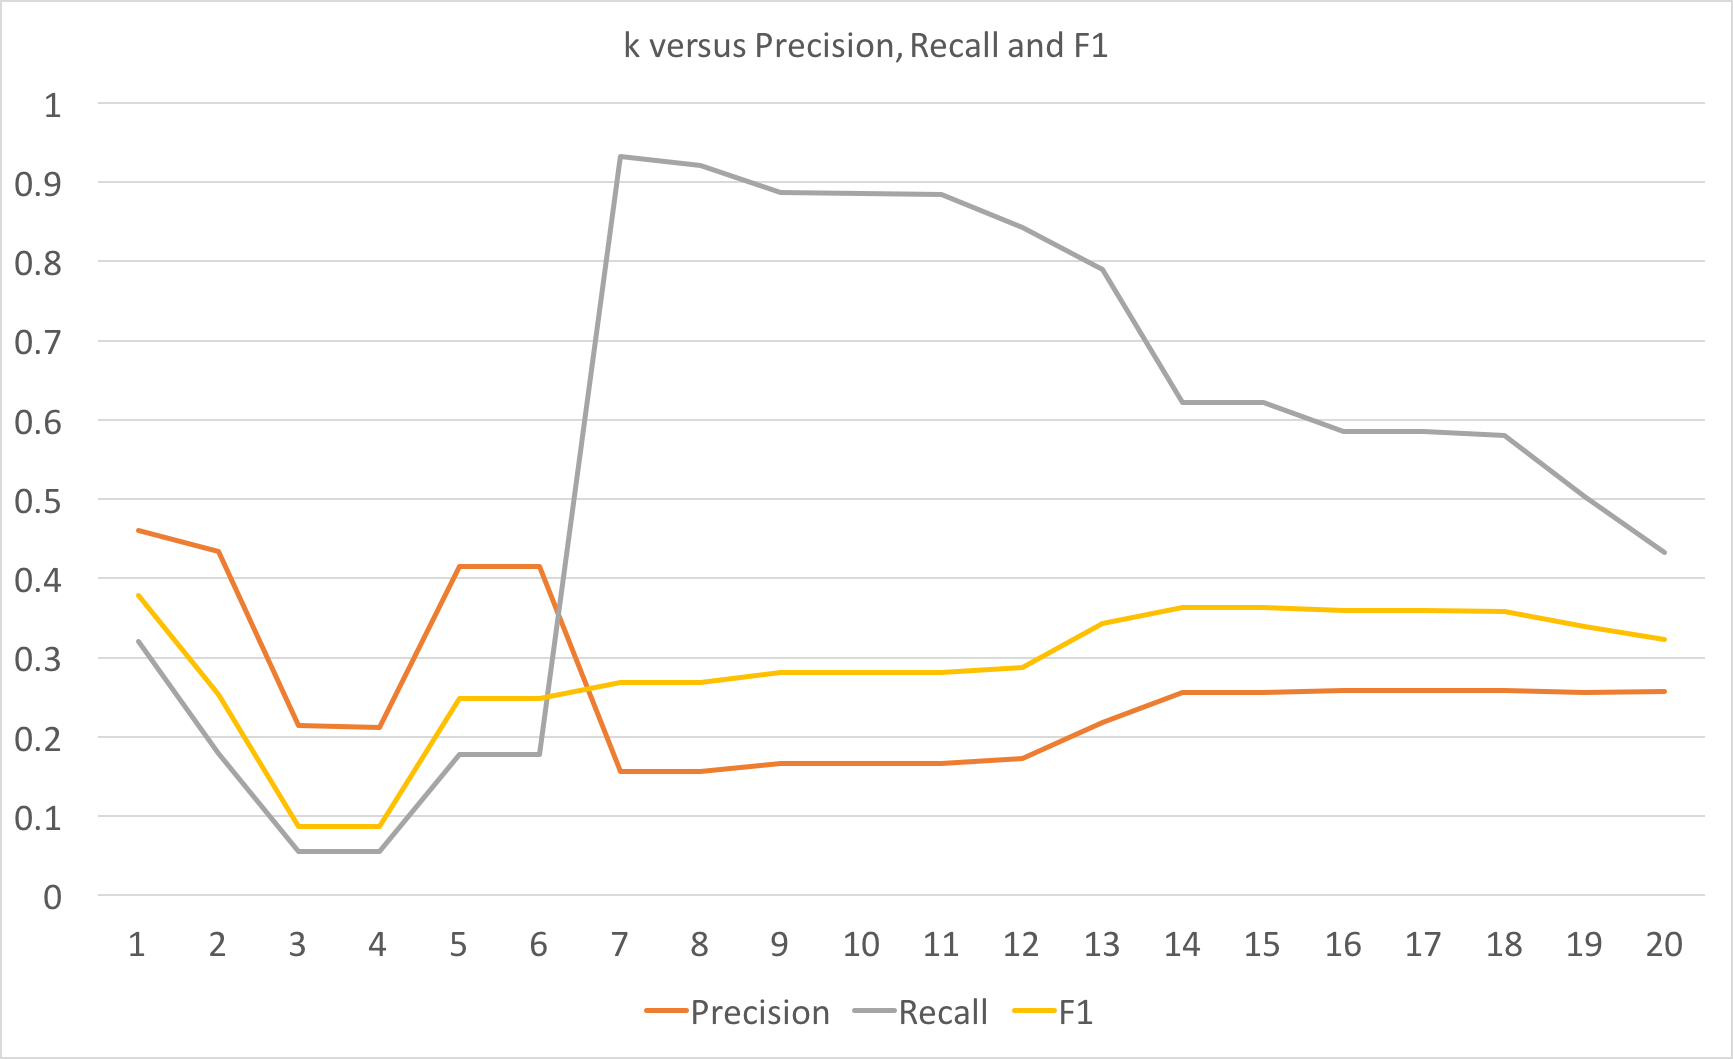
\includegraphics{kBestResults}
			}
			\caption{Results obtained by varying the $k$ parameter in SelectKBest algorithm.}
			\label{fig:kVersusMetrics}
		\end{figure}

	\subsection{Outlier detection and data cleansing}
	
		If one looks at the PDF provided, which was used to create the data set, he will see that two instances, namely ``TOTAL'' and ``THE TRAVEL AGENCY IN THE PARK'' have a very distinct behavior.
		The first instance seems to be the sum of all others and is not a representative example for training, while the second has values in only two of its attributes.
	
		On top of that, all of the employee named ``LOCKHART EUGENE E'' was also removed, since more than 95\% of its attributes were NaNs\footnote{NaN = Not a Number}.
		
		Next, the data set was cleaned by turning all NaN data into $0$ and all negative values into their absolute value, since the data in the provided PDF file has no values below zero.
	
	\subsection{Data scaling}

		Since not all attributes are bounded in the same interval, e.g. most of the e-mail related attributes have a range which is much smaller than the asset ones that might scale way higher, data scaling is needed to make sure that all features have the same weight.
		The procedure adopted for data scaling was simple, which is also the rule of thumb for many books and papers on machine learning.
		The MinMaxScaler from scikit-learn was used to transform features into the $[0;1]$ interval.
		The transformation of an attribute $X$ was done as follows:
		\begin{displaymath}
			\sigma_X = \frac{(X - \min{X})}{\max{X} - \min{X}}
		\end{displaymath}
		\begin{displaymath}
			X_{scaled} = \sigma_X \times (\max{X} - \min{X}) + \min{X}
		\end{displaymath}
		
		Scaling is also important since many learning algorithms, e.g. SGD, Gaussian NB, assume that the data distribution follows a Gaussian distribution.
		Even though the same does not hold for $k$NN, scaling is also important to avoid that too great distances jeopardize distance computations, since a single feature may ``dominate'' the overall distance computation.
		Also, decision tree is able to work with unscaled data, but data scaling was also applied to ease the comparison of the results against the other classifiers.		
		
\section{Results} \label{sec:results}

	This section presents the results obtained in the Enron dataset.
	First, it is detailed how classifier's were tuned, and these tuned versions are then evaluated against one another in three variations of the Enron data set.

	\subsection{Classifier tuning}
	
	
		When applying learning algorithms to different domains, classifiers are likely to act differently.
		Even though researchers try to provide reasonable default parameters, there is no ``one-fits-all''\footnote{Usually referred as the no free lunch theorem.} set of parameters that will succeed in all scenarios.
		Classifier tuning is a step in the machine learning evaluation that compares several different combinations of parameters with the goal of achieving higher classification rates\footnote{In certain scenarios, such as stream processing, the goal could also be to find a fair trade-off between accuracy, processing time and memory usage.}.
		Tuning is in practice a search problem, and thus, many different strategies can be applied to find a fair subset of parameters that maximizes your goal measure.
		In the performed experiments, tuning was performed using a brute force strategy, where all possible combinations of parameters were evaluated with the goal of maximizing the F1-Weighted measure in a 10-fold cross-validation scheme.
		F1-Weighted is a variation of the conventional F1 measure (which is an harmonic mean between the precision and recall and is stated in Equation \ref{eq:f1}) that accounts for instances of each class differently since the problem is unbalanced.
	
		Table \ref{tab:tuningParams} presents the algorithms evaluated and the parameters tuned.
		

	\begin{table*}[!t]
		\centering
		\caption{Algorithms' parameters used for tuning.}
		\resizebox{.7\textwidth}{!}{
		\begin{tabular}{rllll}
			\hline
			Classifier & Parameter & Values tested \\
			\hline
			$k$NN & $k$ & $[1;20]$\\
			~ & $p$\tablefootnote{$p$ is the parameter for the $L_p$ norm, where $L_1$ is the Manhattan distance and $L_2$ is the Euclidian} & $\{1,2,3\}$ \\
			~ & search algorithm & brute\tablefootnote{In my expertise, KDTree approaches are only interesting when we have a high dimensionality data set, which is not the case here, since brute-force search is optimal and not that slow.} \\
			SGD & loss & \{hinge, log, squared\_hinge, perceptron\}\\
			~ & penalty & \{l1, l2, elasticnet\}\\
			Gaussian NB & -- & -- \\
			Decision Tree & Criterion & \{gini, entropy\}\\
			~ & splitter & \{best, random\}\\
			\hline
		\end{tabular}
		}
		\label{tab:tuningParams}
	\end{table*}

	\subsection{Data set variations}
	
		The tuned classifiers are finally compared against one another in four variations of the Enron data set:
		\begin{itemize}
			\item (Original) The original data set, rescaled and without outliers
			\item (New Atts) Original + new attributes
			\item (Selected) New Atts + Feature selection
			\item (Selected + New) Selected + new attributes
		\end{itemize}
		
		These variations will allows a better understanding to the results obtained, since evaluations on how each classifier performs with and without the new attributes and/or feature selection will be possible.
		It is important to highlight that the last variation is used solely to verify the impact of the newly proposed attributes in the results obtained.


	\subsection{Overall evaluation} \label{sec:overallEvaluation}
	
		Validation is one of the most important parts of building and deploying applied machine learning techniques.
		The goal of validation is to verify whether a classifier will predict well when applied in real-world scenarios.
		The rationale behind most of the validation schemes is that the training set and test sets are different, however, built upon the same data generator\footnote{The same does not hold for streaming settings.}.
		Holdout is one of the most simple yet used validation schemes.
		It splits the data set into two disjoint subsets: training and test.
		A classifier is then built using the training set and applied to the test set.
		Even though holdout looks interesting, the test set could be extremely equal or different from the training set, and thus, highly over-fitted or under-fitted results could be obtained.
		To avoid this issue, a 10-fold cross-validation was applied, where a holdout validation was repeated 10 times and the resulting average  is reported.
		Evaluating classifiers using cross-validation is beneficial since it assesses the variability of the results, since it is possible that during one of these folds, classifiers will obtain results that largely deviate from the mean, a fact that should be verified and analyzed.
		It is also worth mentioning that the same procedure was used during feature selection.
						
		Tables \ref{tab:accuracy}, \ref{tab:precision} and \ref{tab:recall} present the results obtained by the tuned classifiers in terms of Accuracy, Precision and Recall, respectively.


		\begin{table*}[!t]
			\centering
			\caption{Average accuracy (\%) obtained in the test script.}
			\resizebox{.7\textwidth}{!}{
			\begin{tabular}{rcccc}
				\hline
				\multicolumn{5}{c}{Accuracy (\%)}\\
				\hline
				Data set & Gaussian NB & $k$NN & SGD & Decision Tree \\
				\hline
				Original & 37.62 & \textbf{87.53} & \textbf{77.35} & 79.87\\
				New Atts & 37.71 & 86.00 & 62.73 & \textbf{80.75} \\
				Selected & \textbf{90.41} & 84.94 & 70.33 & 76.00\\ 
				Selected + New & 83.29 & 82.16 & 55.07 & 78.29 \\
				\hline
			\end{tabular}
			}
			\label{tab:accuracy}
		\end{table*}
	
	
		Verifying the results obtained in accuracy (Table \ref{tab:accuracy}), it is important to highlight that most of the results obtained are below the ZeroR baseline of 88\%, with the exception of the Gaussian Naive Bayes in the Selected data set.
		Another interesting result that should be highlighted is the accuracy increase obtained by the same classifier amongst the data set variations, where the accuracy went from approximately 38\% to 90\%.
		On the other hand, $k$NN, Stochastic Gradient Descent (SGD) and the Decision Tree obtained results below the baseline, however, using the selected subset of attributes decreased the average accuracy obtained.
	
		Besides accuracy, specific metrics for POI recognition should be evaluated.
		To do so, both Precision and Recall metrics were evaluated, and these metrics are computed according to Equations \ref{eq:precision} and \ref{eq:recall}, respectively, where $tp$ are the true positives, $fp$ are the false positives and $fn$ are the false negatives.
		
				
		\begin{equation}
			Precision = \frac{tp}{tp + fp} 
			\label{eq:precision}
		\end{equation} 

		\begin{equation}
			Recall = \frac{tp}{tp + fn}
			\label{eq:recall}
		\end{equation}
		
		\begin{equation}
			F1 = 2 \times \frac{Precision \times Recall}{Precision + Recall}
			\label{eq:f1}
		\end{equation}

		High precision results relates to a low false positive rate (not many false POIs detected), while an high recall relates to a low false negative rate (not many false non-POIs detected).
		Therefore, both precision and recall should be maximized.		
		
		According to the results obtained in Tables \ref{tab:precision} and \ref{tab:recall}, the only classifier able to achieve precision and recall results above 0.3 is the Gaussian Naive Bayes in the selected data set.
		In practice, the results obtained for this combination of classifier and data set shows that it is possible to state that 50\% of the instances flagged as POI by the classifier are really POIs (precision), while 32\% of the POI instances are correctly classified as a POI.
		Again, it is highlighted the last variation of the dataset, which regards the selected features plus the newly generated attributes.
		Focusing on the Gaussian NB results, precision presents an increase of $0.04$ while recall decreases by $0.59$.

		\begin{table*}[!t]
			\centering
			\caption{Average precision obtained in the test script.}
			\resizebox{.7\textwidth}{!}{
			\begin{tabular}{rcccc}
				\hline
				\multicolumn{5}{c}{Precision}\\
				\hline
				Data set & Gaussian NB & $k$NN & SGD & Decision Tree \\
				\hline
				Original & 0.16 & \textbf{0.57} & 0.06 & 0.26 \\
				New Atts & 0.16 & 0.42 & 0.09 & \textbf{0.29} \\
				Selected & 0.46 & 0.40 & 0.12 &  0.16 \\ 
				Selected + New & \textbf{0.50} & 0.34 & \textbf{0.13} & 0.26 \\
				\hline
			\end{tabular}
			}
			\label{tab:precision}		
		\end{table*}
		
		\begin{table*}[!t]
			\centering
			\caption{Average recall obtained in the test script.}
			\resizebox{.7\textwidth}{!}{
			\begin{tabular}{rcccc}
				\hline
				\multicolumn{5}{c}{Recall}\\
				\hline
				Data set & Gaussian NB & $k$NN & SGD & Decision Tree \\
				\hline
				Original & \textbf{0.83} & \textbf{0.27} & 0.04 & 0.28 \\
				New Atts & \textbf{0.83} & 0.13 & 0.19 & \textbf{0.31} \\
				Selected & 0.32 & 0.10 & 0.19 & 0.17 \\ 
				Selected + New & 0.24 & 0.26 & \textbf{0.29} & 0.28 \\
				\hline
			\end{tabular}
			}
			\label{tab:recall}
			
		\end{table*}
	
\end{document}